% \input{"IAB/latex/TeX-Folienformat.tex"}
\input{"/Users/jonathanlatner/Google Drive/My Drive/IAB/latex/TeX-Folienformat.tex"}

\documentclass[t,8pt,utfx8]{beamer}
\usepackage{booktabs}
\usepackage{setspace}
\usepackage{parskip}
\usepackage{graphicx}
\usepackage{subcaption}
\setbeamertemplate{caption}[numbered]
\newcommand{\sprache}{\englisch}
\renewcommand{\thesubsection}{\alph{subsection})}
\usepackage[cal=pxtx, scr=dutchcal]{mathalpha}
\usepackage{forest}



\definecolor{codegreen}{rgb}{0,0.6,0}
\definecolor{codegray}{rgb}{0.5,0.5,0.5}
\definecolor{codepurple}{rgb}{0.58,0,0.82}
\definecolor{backcolour}{rgb}{0.95,0.95,0.92}


\usepackage{listings}

% Define style for R code
\lstset{
  language=R,
  basicstyle=\ttfamily\small,
  keywordstyle=\color{blue},
  stringstyle=\color{red},
  commentstyle=\color{green},
  showstringspaces=false,
  numbers=left,
  numberstyle=\tiny\color{gray},
  stepnumber=1,
  numbersep=5pt,
  breaklines=true,
  frame=single
}

\newcommand{\btVFill}{\vskip0pt plus 1filll}


\title{Buyer Beware: Understanding the trade-off between utility and risk in CART based models using simulation data}

\subtitle{Berlin, \newline 7-8. Oktober, 2024}

\author{Jonathan Latner, PhD \newline Dr. Marcel Neunhoeffer \newline Prof. Dr. Jörg Drechsler}

\newcounter{noauthorlines}
\setcounter{noauthorlines}{2} % Wert für 2 Autoren über 2 Zeilen. Ggf. anpassen

% %%%%%%%%%%%%%%
% Ende Anpassung
% %%%%%%%%%%%%%%

% \input{"IAB/latex/TeX-Folienformatierung_CD_2019"}
\input{"/Users/jonathanlatner/Google Drive/My Drive/IAB/latex/TeX-Folienformatierung_CD_2019"}

% Modify the section in toc template to enumerate
\setbeamertemplate{section in toc}{%
    \inserttocsectionnumber.~\inserttocsection\par
}

% use for subsections
% \setbeamertemplate{subsection in toc}{}
\setbeamertemplate{subsection in toc}{%
    \setlength{\parskip}{1mm}
        \hskip2mm -- \hskip1mm\inserttocsubsection\par
}


\usepackage{colortbl}
\definecolor{lightgray}{gray}{0.9}

\usepackage{listings} %include R code
\lstdefinestyle{mystyle}{
    backgroundcolor=\color{backcolour},   
    commentstyle=\color{codegreen},
    keywordstyle=\color{magenta},
    numberstyle=\tiny\color{codegray},
    stringstyle=\color{codepurple},
    basicstyle=\ttfamily\tiny,
    breakatwhitespace=false,         
    breaklines=true,                 
    captionpos=b,                    
    keepspaces=true,                 
    numbers=left,                    
    numbersep=5pt,                  
    showspaces=false,                
    showstringspaces=false,
    showtabs=false,                 
    columns=fullflexible,
    frame=single,
    tabsize=2
}
\lstset{style=mystyle}


\begin{document}


\frame[plain]{\titlepage}

\begin{spacing}{1.25}


%%%%%%%%%%%%%%%%%%%%%%%%%%%%%%%%%%%%%%%%
%%%%%%%%%%%%%%%%%%%%%%%%%%%%%%%%%%%%%%%%
\section{Introduction}\label{sec:introduction}
%%%%%%%%%%%%%%%%%%%%%%%%%%%%%%%%%%%%%%%%
%%%%%%%%%%%%%%%%%%%%%%%%%%%%%%%%%%%%%%%%

\begin{frame}[c,plain]
\vskip-4mm
\begin{beamercolorbox}[wd=\boxwidth,ht=22.11mm]{transparent}%
    \vfill%
    \usebeamerfont{title}%
    \leftinsert%
    \MakeUppercase{Section \ref{sec:introduction}: Introduction
} % <- Hier die Überschrift eintragen
\end{beamercolorbox}
\vskip-3mm
\pgfuseimage{rahmenlinie}
\end{frame}


\frame{\frametitle{Background}
\begin{itemize}
    \item We think this idea is interesting.
    \item We think others should know about it.
    \item But, this is work in progress.
    \item And, we are still developing it.
    \item Comments and critiques would be helpful.
\end{itemize}
}


\frame{\frametitle{What do we know?}
\begin{itemize}
    \item It is well established that there is a trade-off between utility and privacy when generating synthetic data using a synthetic data generator or SDG (Duncan et al., 2004)
    \item Classification and Regression Trees (CART) models are one type of SDG (Reiter, 2005)
    \begin{itemize}
        \item Utility and privacy in CART based SDGs seems to be high (Little et al., 2022; Danker and Ibrahim, 2021)
        \item Therefore, CART models seem to be less sensitive to this trade-off than other SDGs (i.e. higher utility, lower risk)
    \end{itemize}
\end{itemize}
}

\frame{\frametitle{What do we not know?}
\begin{itemize}
    \item The question: How do CART based SDGs seem to be able to minimize the R-U trade off?
    \begin{itemize}
        \item Relative to other SDGs with certain types of data (i.e. low dimensional data). 
    \end{itemize}
\end{itemize}
}

\frame{\frametitle{What do we do here?}
\begin{itemize}
    \item Using simulation data (Reiter et al., 2014), we show that synthetic data from CART models can be disclosive
    \item {\bf The problem:} Disclosive in ways that are not observable with common privacy metrics
    \item {\bf The solution:} It is possible to increase protection (by reducing utility)
    \item {\bf The question:} Why would we reduce utility if we did not know there was a problem? 
\end{itemize}
}

%%%%%%%%%%%%%%%%%%%%%%%%%%%%%%%%%%%%%%%%
%%%%%%%%%%%%%%%%%%%%%%%%%%%%%%%%%%%%%%%%
\section{The data}\label{sec:data}
%%%%%%%%%%%%%%%%%%%%%%%%%%%%%%%%%%%%%%%%
%%%%%%%%%%%%%%%%%%%%%%%%%%%%%%%%%%%%%%%%
\begin{frame}[c,plain]
\vskip-4mm
\begin{beamercolorbox}[wd=\boxwidth,ht=22.11mm]{transparent}%
    \vfill%
    \usebeamerfont{title}%
    \leftinsert%
    \MakeUppercase{Section \ref{sec:data}: Generate the original and synthetic data
} % <- Hier die Überschrift eintragen
\end{beamercolorbox}
\vskip-3mm
\pgfuseimage{rahmenlinie}

\end{frame}

\frame{\frametitle{Generate original data using a simulation}
\vskip -2mm
\begin{itemize}
    \item Borrowing from Reiter et al. (2014), we create a data set with $n=1000$ and 4 dichotomous, categorical variables. 
    \item The first 999 observations to be a random sample from a multinomial distribution for all combinations of $var1(0,1), var2(0,1), var3(0,1), var4(0,1)$ except the last one
    \item The last (1000$^{th}$) observation is ($var1=1,var2=1,var3=1,var4=1$). 
\end{itemize}



\begin{minipage}{0.48\textwidth}
    \centering
    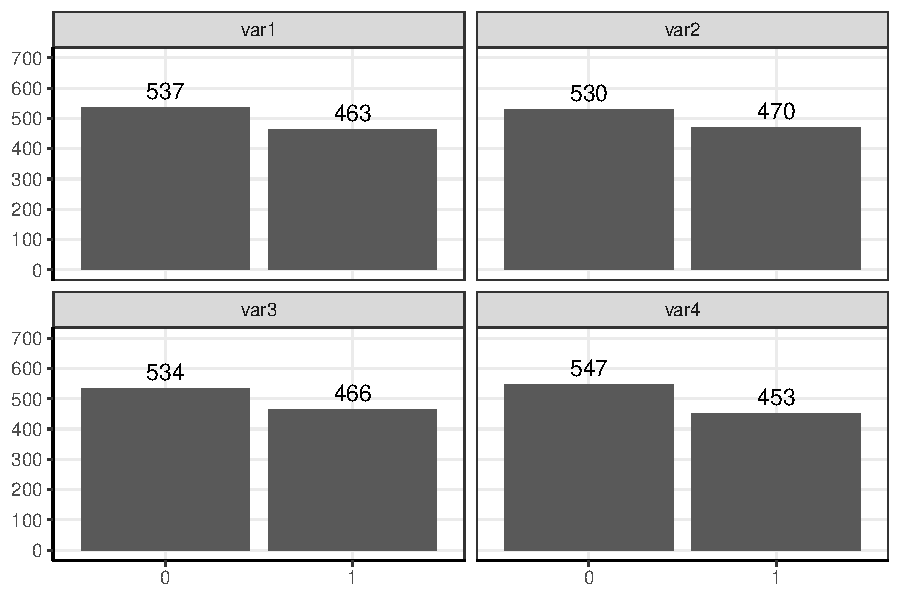
\includegraphics[width=\textwidth]{../../graphs/graph_cart_frequency.pdf}
    % \captionof{figure}{Frequency}
\end{minipage}
\hfill
\begin{minipage}{0.48\textwidth}
    \centering
    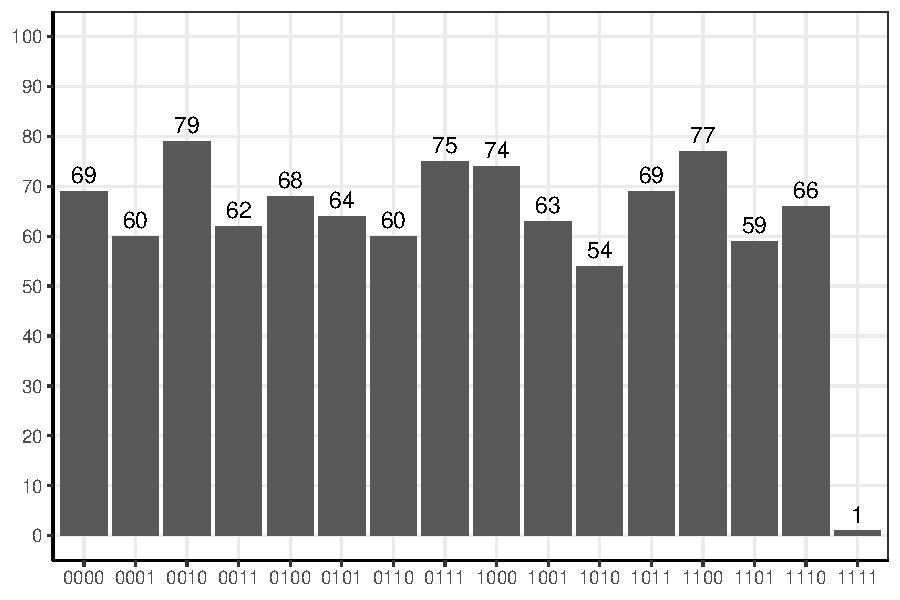
\includegraphics[width=\textwidth]{../../graphs/graph_cart_histogram.pdf}
    % \captionof{figure}{Histogram}
\end{minipage}

}


\frame{\frametitle{Generate synthetic data with CART (synthpop)}

\begin{minipage}{0.48\textwidth}
    \centering
    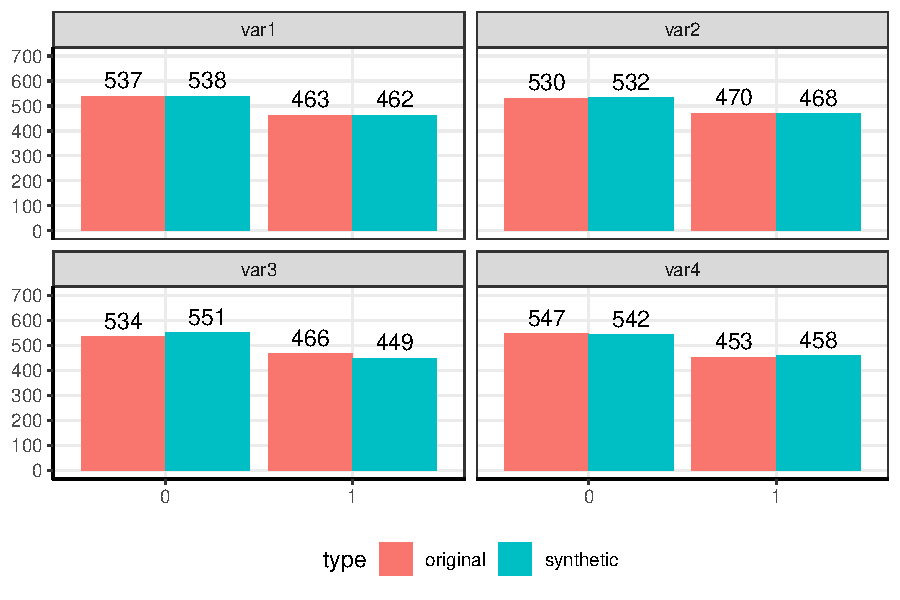
\includegraphics[width=\textwidth]{../../graphs/graph_cart_frequency_compare.pdf}
    \captionof{figure}{Frequency}
\end{minipage}
\hfill
\begin{minipage}{0.48\textwidth}
    \centering
    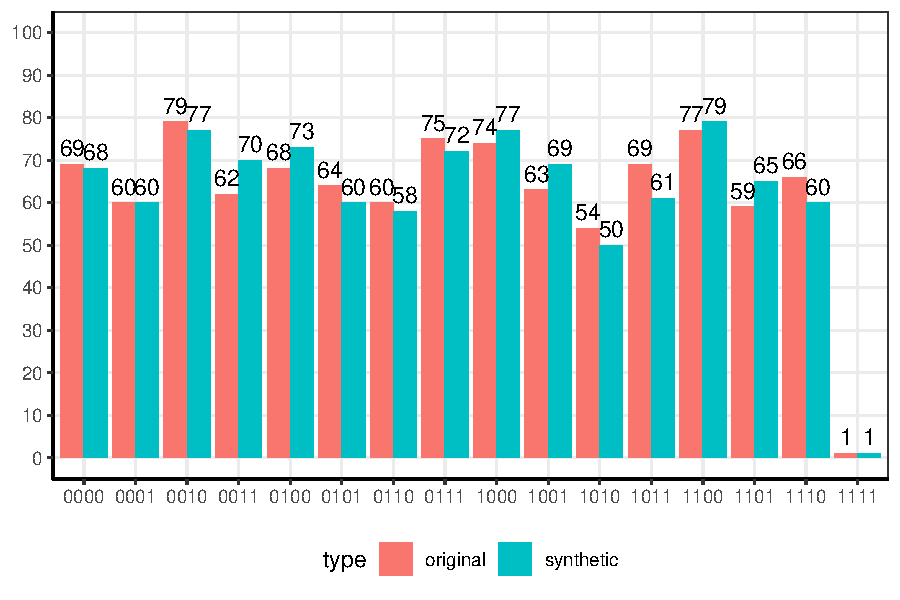
\includegraphics[width=\textwidth]{../../graphs/graph_cart_histogram_compare.pdf}
    \captionof{figure}{Histogram}
\end{minipage}

}


\frame{\frametitle{Compare histogram x 100 synthetic datasets}
\begin{figure}
    \caption{Multiple synthetic data sets does not reduce privacy risk}
    \resizebox{\textwidth}{!}{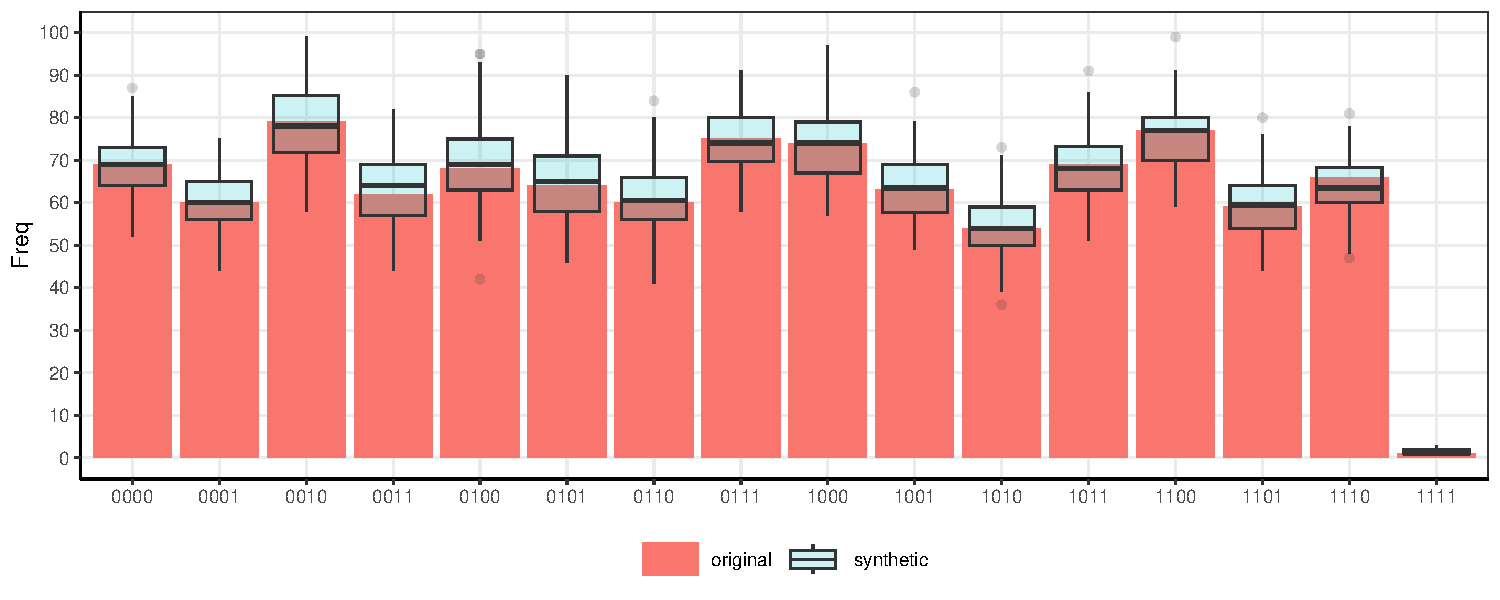
\includegraphics{../../graphs/graph_cart_histogram_compare_100.pdf}}
    \label{fig:graph_cart_histogram_compare_100}
\end{figure}
}

\frame{\frametitle{Summary}
\begin{itemize}
    \item The problem (in our data): Synthetic data from CART models are disclosive
    \item The reason: 
    \begin{itemize}
        \item A record can only be in the synthetic data if it is also in the original data (in this simulated data).   
        \item Or the opposite: if a record is not in the original data, then it can never be in the synthetic data.
    \end{itemize}  
    \item Next section: Can an attacker identify the disclosure?
\end{itemize}
}

%%%%%%%%%%%%%%%%%%%%%%%%%%%%%%%%%%%%%%%%
%%%%%%%%%%%%%%%%%%%%%%%%%%%%%%%%%%%%%%%%
\section{The attack}\label{sec:attack}
%%%%%%%%%%%%%%%%%%%%%%%%%%%%%%%%%%%%%%%%
%%%%%%%%%%%%%%%%%%%%%%%%%%%%%%%%%%%%%%%%
\begin{frame}[c,plain]
\vskip-4mm
\begin{beamercolorbox}[wd=\boxwidth,ht=22.11mm]{transparent}%
    \vfill%
    \usebeamerfont{title}%
    \leftinsert%
    \MakeUppercase{Section \ref{sec:attack}: The attack
} % <- Hier die Überschrift eintragen
\end{beamercolorbox}
\vskip-3mm
\pgfuseimage{rahmenlinie}

\end{frame}

\frame{\frametitle{Setting up the attack}
\begin{itemize}
    \item Its a game between two entities.  
    \begin{itemize}
        \item The statistical agency has the data and wants to release it in a privacy preserving way.  
        \item The attacker wants to identify someone in the data (either membership or attribute inference).  
    \end{itemize}
    \item The question: What can the attacker learn from a released synthetic data set about an individual they do not have knowledge of?
\end{itemize}
}

\frame{\frametitle{Describing the attack}
\begin{itemize}
    \item We assume a `strong' attacker similar to the attack model in differential privacy (DP). 
    \item An attacker has the following knowledge
    \begin{itemize}
        \item Knows the SDG model type (i.e. sequential CART).
        \item Knowledge of all observations in the data except the last one.  
        \item The 16 possible combinations that the last one could be.
    \end{itemize}
    \item The attacker sees the synthetic data
    \item The attacker runs the same synthetic data model (SDG) for all of the 16 different possibilities.  
    \item Then they update their beliefs about what the last record could be
\end{itemize}
}


\frame{\frametitle{Illustrating the attack with CART (default parameters)}
\vskip -3mm
\begin{figure}
    \caption{Histogram of 16 worlds x 100 synthetic datasets}
    \vskip -4mm
    \resizebox{\textwidth}{!}{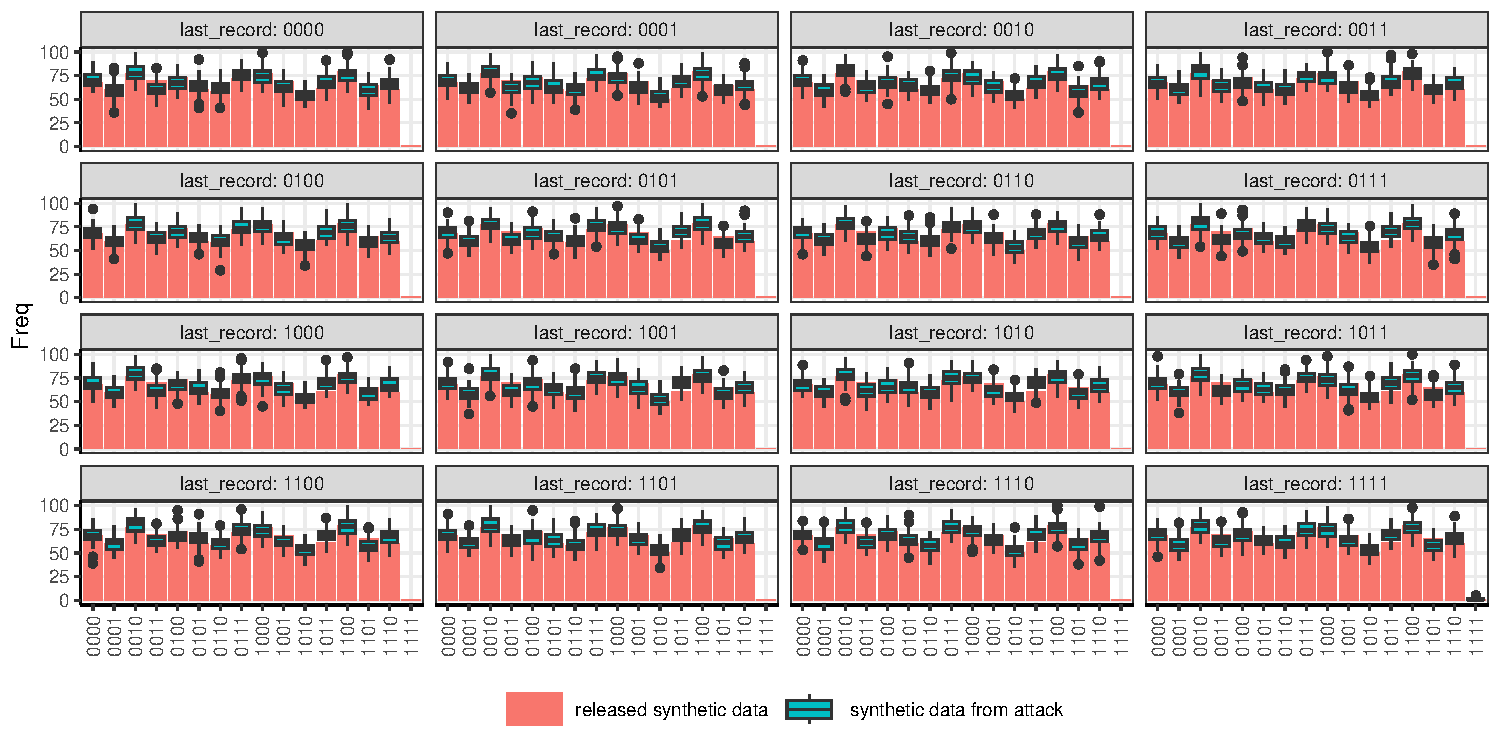
\includegraphics{../../graphs/graph_attacker_default.pdf}}
    \label{fig:graph_attacker_default}
\end{figure}
}


\frame{\frametitle{Summary}
\begin{itemize}
    \item In our attack with our assumptions, the attacker can easily identify the last record
    \item The reason (to repeat): 
    \begin{itemize}
        \item A record can only be in the synthetic data if it is also in the original data (in this simulated data).   
        \item Or the opposite: if a record is not in the original data, then it can never be in the synthetic data.
    \end{itemize}  
    \item Next section: Can we measure this disclosure?
\end{itemize}

}


%%%%%%%%%%%%%%%%%%%%%%%%%%%%%%%%%%%%%%%%
%%%%%%%%%%%%%%%%%%%%%%%%%%%%%%%%%%%%%%%%
\section{Measuring privacy}\label{sec:privacy}
%%%%%%%%%%%%%%%%%%%%%%%%%%%%%%%%%%%%%%%%
%%%%%%%%%%%%%%%%%%%%%%%%%%%%%%%%%%%%%%%%
\begin{frame}[c,plain]
\vskip-4mm
\begin{beamercolorbox}[wd=\boxwidth,ht=22.11mm]{transparent}%
    \vfill%
    \usebeamerfont{title}%
    \leftinsert%
    \MakeUppercase{Section \ref{sec:privacy}: Measuring privacy
} % <- Hier die Überschrift eintragen
\end{beamercolorbox}
\vskip-3mm
\pgfuseimage{rahmenlinie}

\end{frame}


\frame{\frametitle{Privacy measures}
\begin{itemize}
    \item Synthpop (Raab et al., 2024)
    \begin{itemize}
        \item Identity disclosure: the ability to identify individuals in the data from a set of known characteristics (i.e. `keys').
        \item Attribute disclosure: the ability to find out from the keys something, not previously known
        \item Replicated uniques
    \end{itemize}
\end{itemize}
}

\begin{frame}[fragile]
\frametitle{Comparing privacy measures (seed = 1237, i.e. `last record' = 1)}
  
% R Code block


\begin{minipage}[t]{0.48\textwidth}
\begin{lstlisting}
> print(t1, plot = FALSE, to.print = "ident")
Disclosure risk for 1000 records in the original data

Identity disclosure measures
from keys: var1 var2 var3 
For original  ( UiO )  0 %
For synthetic ( repU ) 0 %.
> print(t1, plot = FALSE, to.print = "attrib")

Table of attribute disclosure measures for var1 var2 var3 
Original measure is  Dorig and synthetic measure is DiSCO 
Variables Ordered by synthetic disclosure measure

       attrib.orig attrib.syn check1 Npairs check2
1 var4           0          0             0       
\end{lstlisting}
\end{minipage}%
  \hfill%
\begin{minipage}[t]{0.48\textwidth}
\begin{lstlisting}
> replicated.uniques (sds, df_ods)
    var1 var2 var3 var4
973    1    1    1    1
Uniques and replicated uniques for  1  synthesised data set(s)
 from keys:  var1 var2 var3 var4 

Uniques in  original data:
 1 from  1000 records ( 0.1 %) 
Uniques in synthetic data:
 1 from  1000 records ( 0.1% )

Replicated uniques:
 1
as a % of uniques in synthetic  100%
as a % of original records (repU) 0.1%
\end{lstlisting}
\end{minipage}
\end{frame}

\begin{frame}[fragile]
\frametitle{Comparing privacy measures (seed = 1240, i.e. `last record' = 3)}
  
% R Code block


\begin{minipage}[t]{0.48\textwidth}
\begin{lstlisting}
> print(t1, plot = FALSE, to.print = "ident")
Disclosure risk for 1000 records in the original data

Identity disclosure measures
from keys: var1 var2 var3 
For original  ( UiO )  0 %
For synthetic ( repU ) 0 %.
> print(t1, plot = FALSE, to.print = "attrib")

Table of attribute disclosure measures for var1 var2 var3 
Original measure is  Dorig and synthetic measure is DiSCO 
Variables Ordered by synthetic disclosure measure

       attrib.orig attrib.syn check1 Npairs check2
1 var4           0          0             0       
\end{lstlisting}
\end{minipage}%
  \hfill%
\begin{minipage}[t]{0.48\textwidth}
\begin{lstlisting}
> replicated.uniques (sds, df_ods)
Uniques and replicated uniques for  1  synthesised data set(s)
 from keys:  var1 var2 var3 var4 

Uniques in  original data:
 1 from  1000 records ( 0.1 %) 
Uniques in synthetic data:
 0 from  1000 records ( 0% )

Replicated uniques:
 0
as a % of uniques in synthetic  NaN%
as a % of original records (repU) 0%
\end{lstlisting}
\end{minipage}
\end{frame}

\frame{\frametitle{Summary}
\begin{itemize}
    \item Using common privacy measures, CART generates synthetic data with low risk
    \item 1 measure indicates there may be a problem, but all the other measures indicate there is no problem.
    \item However (and this is the point):
    \begin{itemize}
         \item We know there is a problem (because we created it)
         \item We know that common measures do not capture the problem 
     \end{itemize} 
     % \item We are also not alone in identifying this problem (Manrique-Vallier and Hu, 2018)
\end{itemize}
}


%%%%%%%%%%%%%%%%%%%%%%%%%%%%%%%%%%%%%%%%
%%%%%%%%%%%%%%%%%%%%%%%%%%%%%%%%%%%%%%%%
\section{Solution}\label{sec:solution}
%%%%%%%%%%%%%%%%%%%%%%%%%%%%%%%%%%%%%%%%
%%%%%%%%%%%%%%%%%%%%%%%%%%%%%%%%%%%%%%%%
\begin{frame}[c,plain]
\vskip-4mm
\begin{beamercolorbox}[wd=\boxwidth,ht=22.11mm]{transparent}%
    \vfill%
    \usebeamerfont{title}%
    \leftinsert%
    \MakeUppercase{Section \ref{sec:solution}: Solution
} % <- Hier die Überschrift eintragen
\end{beamercolorbox}
\vskip-3mm
\pgfuseimage{rahmenlinie}
\end{frame}

\frame{\frametitle{The good news: solutions}
\begin{itemize}
    \item Reduce utility by preventing overfitting
    \begin{itemize}
        \item minbucket = 75 (default = 5): increase the minimum number of observations in any terminal node
        \item cp = 0.05 (default = 1e$^{-8}$): decrease the size of the tree
        \item Other options also exist
    \end{itemize}
\end{itemize}
}

\frame{\frametitle{Generate synthetic data with CART (modified parameters)}
\begin{figure}
    \caption{Compare histogram x 100 synthetic datasets}
    \resizebox{\textwidth}{!}{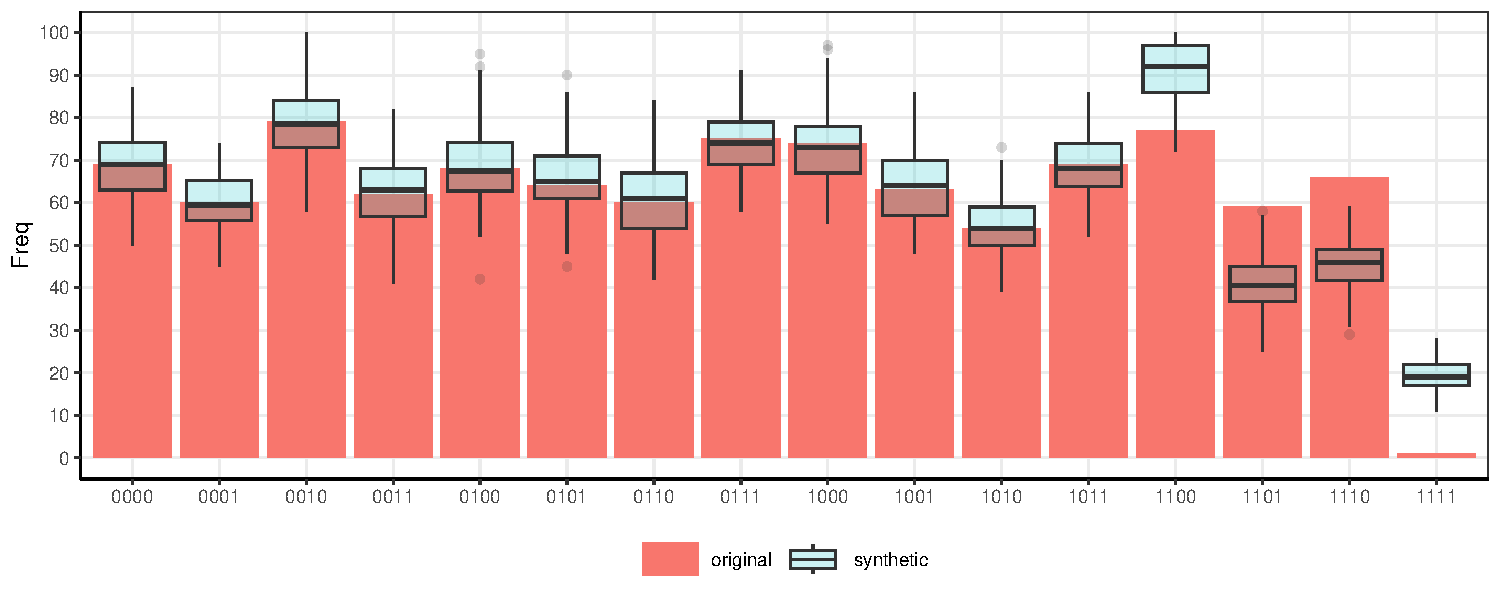
\includegraphics{../../graphs/graph_cart_modified_histogram_compare_100.pdf}}
    \label{fig:graph_cart_modified_histogram_compare_100}
\end{figure}
}


\frame{\frametitle{Illustrating the attack with CART (modified parameters)}
\vskip -3mm
\begin{figure}
    \caption{Histogram of 16 worlds x 100 synthetic datasets}
    \vskip -4mm
    \resizebox{\textwidth}{!}{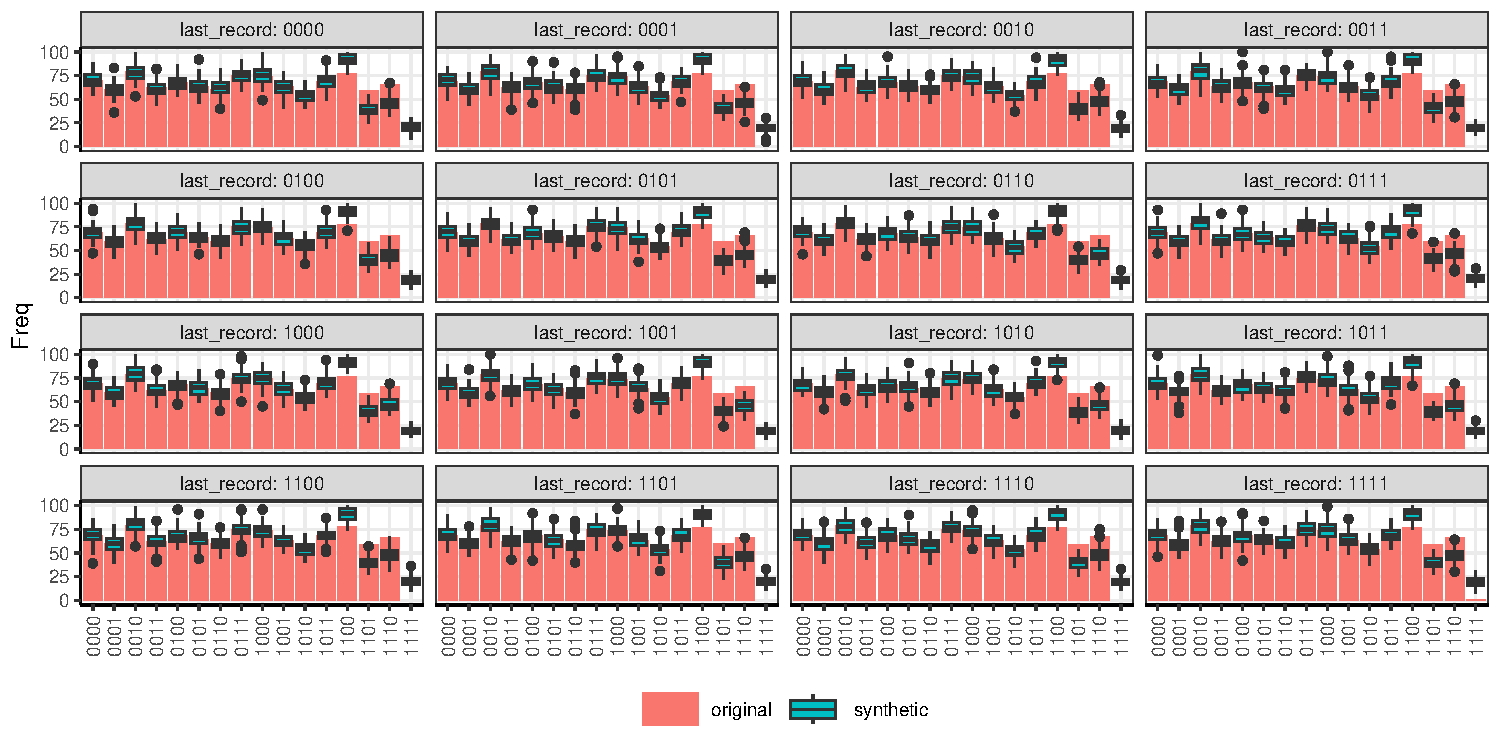
\includegraphics{../../graphs/graph_attacker_modified.pdf}}
    \label{fig:graph_attacker_modified}
\end{figure}
}

\frame{\frametitle{The bad news}
\begin{itemize}
    \item We don't know how to identify the privacy risk
    \item We have to know a problem exists before we would do something about it
\end{itemize}
}

%%%%%%%%%%%%%%%%%%%%%%%%%%%%%%%%%%%%%%%%
%%%%%%%%%%%%%%%%%%%%%%%%%%%%%%%%%%%%%%%%
\section{Conclusion}\label{sec:conclusion}
%%%%%%%%%%%%%%%%%%%%%%%%%%%%%%%%%%%%%%%%
%%%%%%%%%%%%%%%%%%%%%%%%%%%%%%%%%%%%%%%%
\begin{frame}[c,plain]
\vskip-4mm
\begin{beamercolorbox}[wd=\boxwidth,ht=22.11mm]{transparent}%
    \vfill%
    \usebeamerfont{title}%
    \leftinsert%
    \MakeUppercase{Section \ref{sec:conclusion}: Conclusion} % <- Hier die Überschrift eintragen
\end{beamercolorbox}
\vskip-3mm
\pgfuseimage{rahmenlinie}
\end{frame}

\frame{\frametitle{Summary}
\begin{itemize}
    \item It has long been understood that there is a trade-off between utility and risk
    \item Previous research indicated that CART models were less sensitive to this trade-off than other SDGs 
    \item Using a simulated data set, we show that CART are sensitive to this trade-off
    \item The good news: It is possible to reduce risk in CART with parameters
    \item The bad news:
    \begin{itemize}
        \item Common privacy metrics do not capture risk in our simulated data
        \item We must sacrifice utility
    \end{itemize}
    \item Question: If you did not know there was a problem, why would you sacrifice utility?

\end{itemize}
}


\frame{\frametitle{Is the scenario realistic?  Is this a problem?}
\begin{itemize}
    \item No, this is not a problem.  
    \begin{itemize}
        \item A `strong' attacker is unrealistic.
        \begin{itemize}
            \item Knows the SDG model type (i.e. sequential CART).
            \item Knowledge of al observations in the data except the last one.  
            \item The 16 possible combinations that the last one could be.
        \end{itemize}
    \end{itemize}
    \item Yes, this is a problem
    \begin{itemize}
        \item Unique records 
        \begin{itemize}
            \item are always the records we need to protect most
            \item It is well known that SDGs struggle to protect unique records while also providing utility
            \item In this data, eliminating unique records does not solve the problem
        \end{itemize}
        \item The simulation
        \begin{itemize}
            \item We show that a disclosure happened in this data
            \item We show that these risk measures did not capture this disclosure
        \end{itemize}
    \end{itemize}
\end{itemize}
}

\frame{\frametitle{Conclusion}
\begin{itemize}
    \item We are not saying: 
    \begin{itemize}
        \item All synthetic data are disclosive
        \item CART-based SDGs are disclosive
    \end{itemize}
    \item We are saying:
    \begin{itemize}
        \item Do not assume that all risk measures will identify all problems
        \item This simulation offers a type of `bound' on understanding disclosure risks
    \end{itemize}
\end{itemize}
}



\frame{\frametitle{Thank you}

Jonathan Latner: \url{jonathan.latner@iab.de} \\

Reproducible code: \url{https://github.com/jonlatner/KEM\_GAN/tree/main/latner/projects/simulation} 

}



\end{spacing}
\end{document}

